\section{Deadlocks}

A deadlock arises when concurrent transactions hold and request resources held by other transactions.
\begin{definition}[\textit{Lock graph}]
    A lock graph is a bipartite graph in which nodes are resources or transactions and arcs are lock requests or lock assignments. 
\end{definition}
\begin{definition}[\textit{Wait-for graph}]
    A wait-for graph is a graph in which nodes are transactions and arcs are waits for relationships. 
\end{definition}
A deadlock is indicated by a cycle in the wait-for graph of transactions.
\begin{figure}[H]
    \centering
    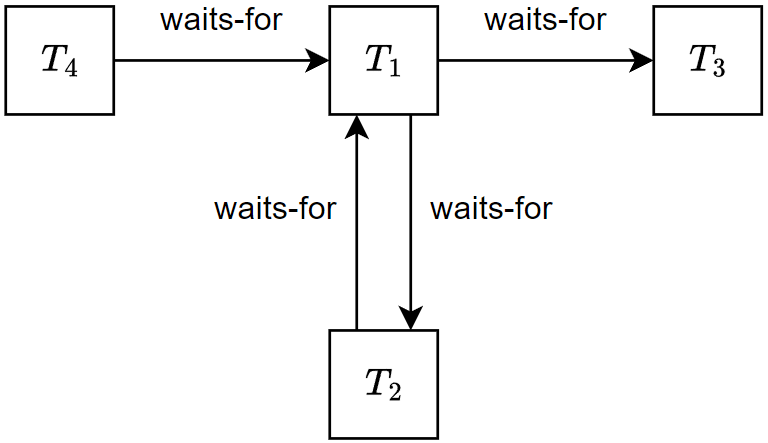
\includegraphics[width=0.5\linewidth]{images/waitgraph.png}
    \caption{An example of deadlock in the wait-for graph}
\end{figure}
It is possible to solve deadlocks in three different ways: 
\begin{itemize}
    \item \textit{Timeout}: a transaction is terminated and restarted after a specified waiting time, determined by the system manager.
    \item \textit{Deadlock prevention}: kills transactions that could cause cycles. 
        It is implemented in two ways: 
        \begin{enumerate}
            \item \textit{Resource-based prevention} puts restrictions on lock requests. 
                The idea is that every transaction requests all resources at once, and only once. 
                The main problem is that it's not easy for transactions to anticipate all requests. 
            \item \textit{Transaction-based prevention} puts restrictions on transactions' IDs. 
                Assigning IDs to transactions incrementally allows to give an age to each one. 
                It is possible to choose to kill the holding transaction (preemptive) or the requesting one (non-preemptive). 
                The main problem is that the number of killings is too big. 
        \end{enumerate}
    \item \textit{Deadlock detection}: it can be implemented with various algorithms and used for distributed resources. 
\end{itemize}

\paragraph*{Dependency graph}
The distributed dependency graph is a wait-for graph where external call nodes represent a sub-transaction activating another sub-transaction at a different node. 
The arrow shows a wait-for relation among local transactions. 
If one term is an external call, either the source is waited for by a remote transaction or waits for a remote transaction. 

\paragraph*{Obermarck's algorithm}
The Obermarck's algorithm needs the following assumptions: 
\begin{itemize}
    \item Transactions execute on a single main node. 
    \item Transactions may be decomposed in sub-transactions running on other nodes. 
    \item When a transaction spawns a sub-transaction it suspends work until the latter completes. 
    \item Two wait-for relationships:
        \begin{itemize}
            \item $T_i$ waits for $T_j$ on the same node because $T_i$ needs a datum locked by $T_j$. 
            \item A sub-transaction of $T_i$ waits for another sub-transaction of $T_i$ running on a different node. 
        \end{itemize}
\end{itemize}
The goal of this algorithm is to detect a potential deadlock looking only at the local view of a node. 
Nodes exchange information and update their local graph based on the received information. 
Node $A$ sends its local info to a node $B$ only if it contains a transaction $T_i$ that is waited for from another remote transaction and waits for a transaction $T_j$ active on $B$ and $i>j$.
\begin{example}
    Consider the given distributed dependency graph:
    \begin{figure}[H]
        \centering
        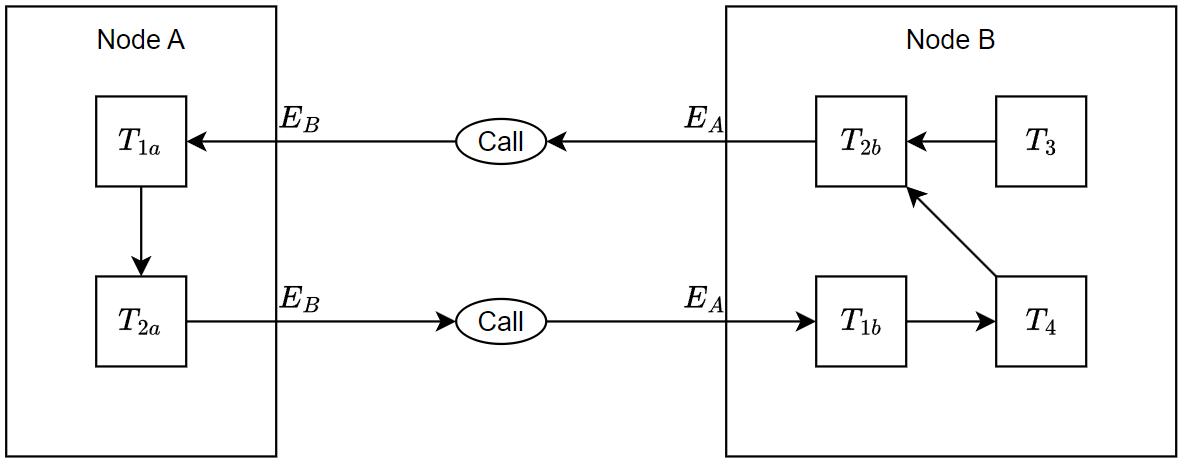
\includegraphics[width=0.5\linewidth]{images/distributedgraph.png}
    \end{figure}
    In this graph, a potential deadlock is indicated by cycles.
    Specifically, we observe that $T_{2a}$ waits for $T_{1a}$ (data lock), which, in turn, waits for $T_{1b}$ (call), leading to a sequence where $T_{2b}$ (data locks) waits for $T_{2a}$ (call).
    
    In this case the node $A$ dispatches information to $B$, in fact we have $ E_b \rightarrow T_2 \rightarrow T_1 \rightarrow E_b$ and node $B$ cannot dispatch information to $A$, because the forwarding rule is not respected: $E_a \rightarrow T_1 \rightarrow T_2 \rightarrow E_a$. 
\end{example}
The Obermarck's algorithm runs periodically at each node and consists in four steps: 
\begin{enumerate}
    \item Obtain graph info from the previous nodes.
    \item Update the local graph by merging the received information.
    \item Check for cycles among transactions, indicating potential deadlocks. 
        If found, select one transaction in the cycle and terminate it.
    \item Send the updated graph info to the next nodes.
\end{enumerate}
\begin{example}
    Given the following distributed system:
    \begin{figure}[H]
        \centering
        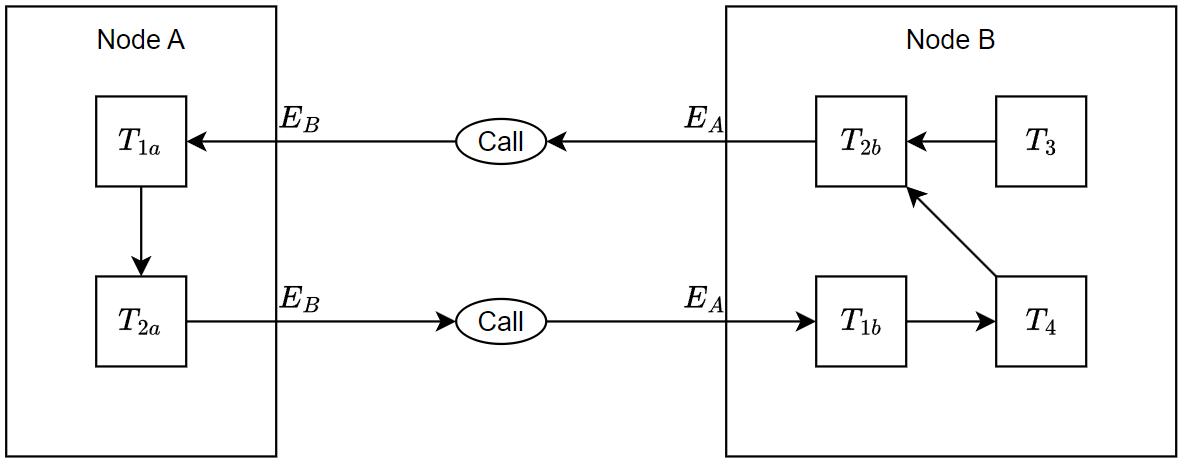
\includegraphics[width=0.5\linewidth]{images/distributedgraph.png}
    \end{figure}
    Let's apply the Obermarck's algorithm:
    \begin{enumerate}
        \item Use the forwarding rule, in this case we have: 
            \begin{itemize}
                \item At Node $A$: $E_b \rightarrow T_2 \rightarrow T_1 \rightarrow E_b$ info sent to Node $B$
                \item At Node $B$: $E_a \rightarrow T_1 \rightarrow T_2 \rightarrow E_a$ info not sent $(i<j)$. 
            \end{itemize}
        \item At node $B$ there is the updated info $E_b \rightarrow T_2 \rightarrow T_1 \rightarrow E_b$. and it is added to the wait-for graph.
        \item At node $B$ a deadlock is detected (cycle between $T_1$ and $T_2$) and $T_1$, $T_2$ or $T_4$ are killed. 
        \item Updated information are sent to all nodes. 
    \end{enumerate}
\end{example}
Four variants based on different conventions regarding message conditions and receivers.
\begin{table}[H]
    \centering
    \begin{tabular}{c|cc|}
    \cline{2-3}
    \textbf{}               & \textbf{Message condition} & \textbf{Message receiver} \\ \hline
    \multicolumn{1}{|l|}{A} & $i>j$                      & Following node            \\
    \multicolumn{1}{|l|}{B} & $i>j$                      & Preceding node            \\
    \multicolumn{1}{|l|}{C} & $i<j$                      & Following node            \\
    \multicolumn{1}{|l|}{D} & $i<j$                      & Preceding node            \\ \hline
    \end{tabular}
\end{table}

\paragraph*{Practical application}
In practical scenarios, the likelihood of encountering deadlocks ($n^{-2}$) is considerably lower than the probability of conflicts ($n^{-1}$).
Various techniques are employed to minimize the occurrence of deadlocks:
\begin{itemize}
    \item \textit{Update lock}: the most frequent deadlock occurs when two concurrent transactions start by reading the same resources and then decide to write and try to upgrade their lock to write on the resource. 
    To avoid this situation, systems offer the update lock, that is used by transactions that will read and then write. 
    The lock table become: 
    \begin{table}[H]
        \centering
        \begin{tabular}{ccccc}
        \textbf{}                                     & \multicolumn{4}{c}{\textbf{Resource status}}                                                                                                        \\ \cline{2-5} 
        \multicolumn{1}{c|}{\textbf{Request}}         & \textit{FREE}                     & \textit{SHARED}                   & \textit{UPDATE}                   & \multicolumn{1}{c|}{\textit{EXCLUSIVE}} \\ \hline
        \multicolumn{1}{|c|}{\textit{Shared lock}}    & \multicolumn{1}{c}{$\checkmark$} & \multicolumn{1}{c}{$\checkmark$} & \multicolumn{1}{c}{$\checkmark$} & \multicolumn{1}{c|}{$\tikzxmark$}       \\ 
        \multicolumn{1}{|c|}{\textit{Update lock}}    & \multicolumn{1}{c}{$\checkmark$} & \multicolumn{1}{c}{$\checkmark$} & \multicolumn{1}{c}{$\tikzxmark$} & \multicolumn{1}{c|}{$\tikzxmark$}       \\ 
        \multicolumn{1}{|c|}{\textit{Exclusive lock}} & \multicolumn{1}{c}{$\checkmark$} & \multicolumn{1}{c}{$\tikzxmark$} & \multicolumn{1}{c}{$\tikzxmark$} & \multicolumn{1}{c|}{$\tikzxmark$}       \\ \hline
        \end{tabular}
    \end{table}
    \item \textit{Hierarchical lock}: locks can be specified with different granularity. 
        The objective of this is to lock the minimum amount of data and recognize conflicts as soon as possible.
        The method used to do so consists in asking locks on hierarchical resources by requesting resources top-down until the right level is obtained and releasing locks bottom-up. 
        This is done by using five locking modes: shared, exclusive, ISL (intention of locking a sub-element of the current element in shared mode), IXL (intention of locking a sub-element of the current element in exclusive mode), and SIXL (lock of the element in shared mode with intention of locking a sub-element in exclusive mode). 
        The lock table is modified as follows:
    \begin{table}[H]
        \centering
        \begin{tabular}{ccccccc}
        \textbf{}                             & \multicolumn{6}{c}{\textbf{Resource status}}                                                                                                                                                                            \\ \cline{2-7} 
        \multicolumn{1}{c|}{\textbf{Request}} & \multicolumn{1}{c}{\textit{FREE}} & \multicolumn{1}{c}{\textit{ISL}} & \multicolumn{1}{c}{\textit{IXL}} & \multicolumn{1}{c}{\textit{SL}}  & \multicolumn{1}{c}{\textit{SIXL}} & \multicolumn{1}{c|}{\textit{XL}}  \\ \hline
        \multicolumn{1}{|c|}{\textit{ISL}}    & \multicolumn{1}{c}{$\checkmark$}  & \multicolumn{1}{c}{$\checkmark$} & \multicolumn{1}{c}{$\checkmark$} & \multicolumn{1}{c}{$\checkmark$} & \multicolumn{1}{c}{$\checkmark$}  & \multicolumn{1}{c|}{$\tikzxmark$} \\ 
        \multicolumn{1}{|c|}{\textit{IXL}}    & \multicolumn{1}{c}{$\checkmark$}  & \multicolumn{1}{c}{$\checkmark$} & \multicolumn{1}{c}{$\checkmark$} & \multicolumn{1}{c}{$\tikzxmark$} & \multicolumn{1}{c}{$\tikzxmark$}  & \multicolumn{1}{c|}{$\tikzxmark$} \\ 
        \multicolumn{1}{|c|}{\textit{SL}}     & \multicolumn{1}{c}{$\checkmark$}  & \multicolumn{1}{c}{$\checkmark$} & \multicolumn{1}{c}{$\tikzxmark$} & \multicolumn{1}{c}{$\checkmark$} & \multicolumn{1}{c}{$\tikzxmark$}  & \multicolumn{1}{c|}{$\tikzxmark$} \\
        \multicolumn{1}{|c|}{\textit{SIXL}}   & \multicolumn{1}{c}{$\checkmark$}  & \multicolumn{1}{c}{$\checkmark$} & \multicolumn{1}{c}{$\tikzxmark$} & \multicolumn{1}{c}{$\tikzxmark$} & \multicolumn{1}{c}{$\tikzxmark$}  & \multicolumn{1}{c|}{$\tikzxmark$} \\ 
        \multicolumn{1}{|c|}{\textit{XL}}     & \multicolumn{1}{c}{$\checkmark$}  & \multicolumn{1}{c}{$\tikzxmark$} & \multicolumn{1}{c}{$\tikzxmark$} & \multicolumn{1}{c}{$\tikzxmark$} & \multicolumn{1}{c}{$\tikzxmark$}  & \multicolumn{1}{c|}{$\tikzxmark$} \\ \hline
        \end{tabular}
    \end{table}
    \begin{example}
        Given a table $X$ with eight tuples divided in two pages: 
        \begin{table}[H]
            \centering
            \begin{tabular}{cc}
            \textbf{P1}                 & \textbf{P2}               \\ \hline
            \multicolumn{1}{|c|}{$t1$}  & \multicolumn{1}{c|}{$t5$} \\ 
            \multicolumn{1}{|c|}{$t2$}  & \multicolumn{1}{c|}{$t6$} \\ 
            \multicolumn{1}{|c|}{$t3$}  & \multicolumn{1}{c|}{$t7$} \\ 
            \multicolumn{1}{|c|}{$t4$}  & \multicolumn{1}{c|}{$t8$} \\ \hline
            \end{tabular}
        \end{table}
        And two transactions with the following schedules: 
        \[T_1=r(P1)\:w(t3)\:r(t8)\]
        \[T_2=r(t2)\:r(t4)\:w(t5)\:w(t6)\]
        We can see that they are not in a read-write conflict (because they are independent of the order). 
        Without hierarchical locking both transactions needs to operate on the same table, so the concurrency will be almost useless in this case. 
        But with this technique, calling $X$ the table, we have that the transaction acquires the following locks: 
        \[T_1:\:\textnormal{IXL}(root)\:\textnormal{SIXL}(P1)\:\textnormal{XL}(t3)\:\textnormal{ISL}(P2)\:\textnormal{SL}(t8)\]
        \[T_2:\:\textnormal{IXL}(root)\:\textnormal{ISL}(P1)\:\textnormal{SL}(t2)\:\textnormal{SL}(t4)\:\textnormal{IXL}(P2)\:\textnormal{XL}(t5)\:\textnormal{XL}(t6)\]
    \end{example}
\end{itemize}